%========================
% Document class and theme
%========================
\documentclass[8pt]{beamer}
\usetheme[progressbar=frametitle]{metropolis}
\setbeamersize{text margin left=10mm, text margin right=10mm}
\usepackage{appendixnumberbeamer} % appendix slide numbering
\setbeamertemplate{theorems}[numbered]

%========================
% Core packages
%========================
\usepackage{amsmath, amsfonts, amssymb, amsthm} % math + theorems
\usepackage{booktabs}        % professional tables
\usepackage{hyperref}        % hyperlinks
\usepackage{xcolor}          % colors
\usepackage{xspace}          % spacing for custom commands

%========================
% Algorithms
%========================
\usepackage{algorithm}
\usepackage{algpseudocode}
\newtheorem{proposition}{Proposition}

%========================
% Plots and TikZ
%========================
\usepackage{pgfplots}
\usepgfplotslibrary{dateplot}
\usepackage{tikz}
\usetikzlibrary{positioning}

%========================
% Listings (code)
%========================
\usepackage{listings}
\lstset{
    basicstyle=\ttfamily\small,
    breaklines=true,
    numbers=left,
    numberstyle=\tiny
}

% R style
\lstdefinelanguage{R}{
  morekeywords={TRUE,FALSE},
  deletekeywords={data,frame,length,as,character},
  otherkeywords={0,1,2,3,4,5,6,7,8,9},
  keywordstyle=\color{blue},
  commentstyle=\color{DarkGreen},
  stringstyle=\color{DarkGreen},
  basicstyle=\ttfamily\small
}

% Python style
\lstdefinelanguage{PythonCustom}{
  language=Python,
  keywordstyle=\color{blue},
  commentstyle=\color{gray},
  stringstyle=\color{red},
  basicstyle=\ttfamily\small
}

%========================
% Custom commands
%========================
\newcommand{\themename}{\textbf{\textsc{metropolis}}\xspace}

%========================
% Custom footline
%========================
\setbeamertemplate{footline}
{%
  \leavevmode%
  \hbox{%
  \begin{beamercolorbox}[wd=.35\paperwidth,ht=2.5ex,dp=1.5ex,center]{author in head/foot}%
    \usebeamerfont{author in head/foot}\insertshortauthor
  \end{beamercolorbox}%
  \begin{beamercolorbox}[wd=.3\paperwidth,ht=2.5ex,dp=1ex,center]{title in head/foot}%
    \usebeamerfont{title in head/foot}\insertshorttitle
  \end{beamercolorbox}%
  \begin{beamercolorbox}[wd=.3\paperwidth,ht=2.5ex,dp=1ex,right]{date in head/foot}%
    \usebeamerfont{date in head/foot}\insertframenumber{} / \inserttotalframenumber
  \end{beamercolorbox}}%
  \vskip0pt%
}

%========================
% Beamer tweaks
%========================
\setbeamertemplate{navigation symbols}{} % remove default navigation symbols


%%%%%%%%%%%%%%%%%%%%%%%%%%%%%%%%%%%%%%%%%%%%%%%%%%%%%%%%%%%%%%%%%%%%
%%%%%%%%%%%%%%%%%%%%%%%%%%%%%%%%%%%%%%%%%%%%%%%%%%%%%%%%%%%%%%%%%%%%
% AQUI SE DEFINEN LAS IMAGENES PARA UTILIZAR DESPUES
%\pgfdeclareimage[interpolate=true, height=7cm,width=16cm]{halton-points}{halton-points}
%\pgfdeclareimage[interpolate=true, height=3cm, width =4cm]
%{serie-petroleo-reducido}{serie-petroleo-reducido}
%\pgfdeclareimage[interpolate=true, height=3cm, width =4cm]{rectangle-triangle}{rectangle-triangle}
%\pgfdeclareimage[interpolate=true, height=3cm, width =4cm]{any-angle}{any-angle}
%\pgfdeclareimage[interpolate=true, height=3cm, width =4cm]{Pythagoras}{Pythagoras}


\title{Chapter 2 - Simulating Statistical Models}
\subtitle{Markov Chains.}
\author{Prof. Alex Alvarez, Ali Raisolsadat}
\institute{School of Mathematical and Computational Sciences \\ University of Prince Edward Island}
\date{} % leave empty or add \today
%\title[Stat 4110]{Stat 4110 Statistical Simulation}
%\subtitle{}
%\author[University of Prince Edward Island]{School of Mathematical and Computational Sciences \\ University of Prince Edward Island}

%========================
% Begin document
%========================
\begin{document}

%-------------------
% Title frame
%-------------------
\maketitle


%-------------------
% Slide 1: Stochastic Process
%-------------------
\begin{frame}{Stochastic Process}
\begin{block}{Definition}
A \textbf{stochastic process} is a collection of random variables
\begin{equation*}
X = \{ X_t \}_{t \in T}, \quad X_t \in S
\end{equation*}
where
\begin{itemize}
  \item $T$ = \textbf{index set} (often time: $\mathbb{N}$ for discrete, $\mathbb{R}^+$ for continuous) 
  \item $S$ = \textbf{state space} (possible values of $X_t$)
\end{itemize}
\end{block}

\begin{exampleblock}{Examples}
\begin{itemize}
  \item Tossing a coin repeatedly: $X_t \in \{0,1\}$ 
  \item Daily stock price: $X_t \in \mathbb{R}^+$
  \item Temperature over time: $X_t \in \mathbb{R}$
\end{itemize}
\end{exampleblock}

\begin{alertblock}{Key Idea}
\vspace{1mm}
The random variables $X_t$ are usually \textbf{dependent}, and interesting processes have \emph{structured dependence}.
\end{alertblock}
\end{frame}

%-------------------
% Slide 2: Dependence Structure
%-------------------
\begin{frame}{Dependence Structure}
\begin{block}{Classical Assumption}
Many results in probability theory assume that random variables are 
\textbf{independent}, which makes computations much easier.
\end{block}

\begin{exampleblock}{But in Reality...}
\begin{itemize}
  \item Independence is often \textbf{not realistic} 
        (e.g., stock prices, weather, genetics).  
  \item Random variables are usually \textbf{dependent}.
\end{itemize}
\end{exampleblock}

\begin{alertblock}{The Challenge}
\vspace{1mm}
Therefore, adding dependence between random variables makes computations more difficult.  
\newline
\newline
\textbf{Goal:} Find dependence structures that are both \textbf{realistic and computationally workable}.
\end{alertblock}

\vspace{2mm}

\begin{block}{BEHOLD: The most awesome Markov Chains}
\vspace{1mm}
They provide a \alert{simple yet powerful model of dependence}: the future depends only on the present, not on the entire past.
\end{block}
\end{frame}

%-------------------
% Slide 3: Dependence Structure
%-------------------
\begin{frame}{Dependence in a Markov Chain}
\begin{block}{Intuition} 
\vspace{1mm}
A Markov chain has \textbf{no memory}. That is to say that the \textbf{most recent state} only matters for predicting the next one.
\end{block}

\vspace{2mm}

\begin{definition}[Discrete-Time Markov Chain]
\vspace{1mm}
A stochastic process 
\begin{equation*}
X = \{X_0, X_1, X_2, \ldots\}, \quad X_n \in S
\end{equation*}
satisfies the \textbf{Markov property} if for all $n \geq 0$,
\begin{equation*}
P(X_{n+1} \in A_j \mid X_0=i_0, X_1=i_1, \ldots, X_n=i_n) 
= P(X_{n+1} \in A_j \mid X_n = i_n).
\end{equation*}
\end{definition}

\vspace{2mm}

\begin{exampleblock}{Notes}
\begin{itemize}
  \item The distribution of $X_0$ is called the \textbf{initial distribution}.  
  \item Sometimes $X_0$ is known (and not random).  
  \item The condition above is called the \textbf{Markov property}, 
        named after Russian mathematician Andrey Markov.
\end{itemize}
\end{exampleblock}
\end{frame}

% --------------------------
% Slide 4: Random walk definition
% --------------------------
\begin{frame}{Simple Random Walk (definition)}
\begin{block}{Simple random walk}
\vspace{1mm}
Let \(\{Y_k\}_{k\ge 1}\) be i.i.d.\ random variables (``steps'') with
\begin{equation*}
\mathbb{P}(Y_k = 1) = p,\qquad \mathbb{P}(Y_k = -1) = 1-p
\end{equation*}
Fix an initial state \(X_0\in\mathbb{Z}\). Define the \emph{random walk}
\begin{equation*}
X_n = X_0 + \sum_{k=1}^n Y_k,\qquad n\ge1
\end{equation*}
Thus each step moves the walker by \(+1\) or \(-1\).
\end{block}

\begin{exampleblock}{Intuition}
The next position \(X_{n+1}\) is obtained by adding one fresh independent step \(Y_{n+1}\) to the current position \(X_n\).
\end{exampleblock}

\begin{proposition}
The random walk \(\{X_n\}\) defined above satisfies the Markov property:
for all \(n\ge0\) and integers \(i_0,\dots,i_n,j\),
\begin{equation*}
\mathbb{P}(X_{n+1}=j\mid X_0=i_0,\dots,X_n=i_n)
=\mathbb{P}(X_{n+1}=j\mid X_n=i_n)
\end{equation*}
\end{proposition}
\end{frame}

% --------------------------
% Sldie 5: Example-based proof of Markov property
% --------------------------
\begin{frame}{Random Walk $\Rightarrow$ Markov Property (example-based proof)}
\textbf{Proof}.
Start from the left-hand conditional probability and use the construction \(X_{n+1}=X_n+Y_{n+1}\):
\begin{equation*}
\begin{aligned}
\mathbb{P}(X_{n+1}=j\mid X_0=i_0,\dots,X_n=i_n)
&= \mathbb{P}(i_n + Y_{n+1} = j \mid X_0=i_0,\dots,X_n=i_n)\\[4pt]
&= \mathbb{P}(Y_{n+1}=j-i_n \mid X_0=i_0,\dots,X_n=i_n).
\end{aligned}
\end{equation*}
Because \(Y_{n+1}\) is independent of the past (the \(\{Y_k\}\) are i.i.d.),
the conditioning on \(X_0,\dots,X_n\) is irrelevant, so
\begin{equation*}
\mathbb{P}(Y_{n+1}=j-i_n \mid X_0,\dots,X_n)
= \mathbb{P}(Y_{n+1}=j-i_n).
\end{equation*}
\end{frame}

% --------------------------
% Sldie 6: Example of Markov property
% --------------------------
\begin{frame}{Why the Markov Property Holds (Random Walk Example)}
The event $\{X_{n+1}=j\}$ is the same as
\begin{equation*}
\{\,i_n + Y_{n+1} = j\,\} 
\quad \Longleftrightarrow \quad
\{\,Y_{n+1} = j - i_n\,\}
\end{equation*}
Thus,
\begin{equation*}
\mathbb{P}(X_{n+1}=j \mid X_n=i_n) 
= \mathbb{P}(Y_{n+1}=j-i_n)
\end{equation*}
Since $Y_{n+1}$ is independent of the past, the history $(X_0,\dots,X_{n-1})$ does not matter. Hence the Markov property holds all \(n\ge0\) and integers \(i_0,\dots,i_n,j\). 
\end{frame}

% --------------------------
% Sldie 7: Example of Markov property
% --------------------------
\begin{frame}{Why the Markov Property Holds -- Example}
\textbf{A Gambler's Fortune.}  
Let $X_n$ be the amount of money a gambler has after $n$ bets.  
At each step:
\begin{equation*}
X_{n+1} = X_n + Y_{n+1}, \quad 
Y_{n+1} =
\begin{cases}
\text{heads} & \text{(win \$1)} \\
\text{tails} & \text{(lose \$1)} 
\end{cases}
\end{equation*}

If the gambler currently has \$10, then the next outcome depends only on the result of the next bet ($Y_{n+1}$), not on how they got to \$10.  

But we can still see that for an unbiased coin ($p = \frac{1}{2}$)
\begin{equation*}
P(X_{n} > 10) = \sum_{k = \lfloor n/2 \rfloor + 1}^{n} \binom{n}{k}\biggl(\frac{1}{2}\biggl)^{n}; \quad P(X_{n} > 10) \approx \frac{1}{2} \quad \text{as $n \rightarrow \infty $; by CLT}
\end{equation*}

\begin{block}{Takeaway}
The process is Markov because the \emph{future fortune depends only on the present fortune and the next bet}, not the entire betting history.
\end{block}
\end{frame}

% --------------------------
% Sldie 8: Markov Property Discussion
% --------------------------
\begin{frame}{Markov Property Discussion}
\textbf{Interpretation:}  
The future is independent of the past \alert{given the present}.  

\bigskip

\begin{itemize}
  \item Natural in many applications:
    \begin{itemize}
      \item Total gains/losses in gambling
      \item Cumulative processes such as queues
    \end{itemize}
  
  \bigskip
  
  \item The Markov property makes probability calculations much easier:
    \begin{itemize}
      \item Compute probabilities and expectations step by step
      \item No need to assume all random variables are independent
    \end{itemize}
\end{itemize}
\end{frame}


% --------------------------
% Sldie 9: Homogeneous Markov Chain
% --------------------------
\begin{frame}{Homogeneous Markov Chain}
Let us  consider first the case of finite/discrete state space $S$.

\vspace{3mm}

Conditional probabilities of the type $P(X_{n+1}=j|X_n=i)$ are called  one-step transition probabilities \textbf{from state $i$ to state $j$}.
\vspace{3mm}

If these one-step transition probabilities do not depend on time variable $n$, then
we say that the Markov Chain is \textbf{homogeneous} and we write:
\begin{equation*}
P(X_{n+1}=j|X_n=i)=p_{ij}
\end{equation*}
\end{frame}

% --------------------------
% Slide 10: Calculating probabilities
% --------------------------
\begin{frame}{Homogeneous Markov Chain}
\textbf{Calculating probabilities}

\vspace{3mm}

If the Markov chain is homogeneous, we have:

\begin{eqnarray*}
&&P(X_0=i_0,X_1=i_1,\ldots,X_{n+1}=i_{n+1})\\
&=&\displaystyle{P(X_0=i_0) \cdot \prod_{k=0}^n P(X_{k+1}=i_{k+1}|X_k=i_k)}\\
&=&\displaystyle{P(X_0=i_0) \cdot \prod_{k=0}^n p_{i_k i_{k+1}}}\\
\end{eqnarray*}

\vspace{3mm}

The probabilities of the whole trajectories of the Markov Chain is determined by the transition probabilities and the initial distribution of $X_0$.
\end{frame}

% --------------------------
% Slide 11: Transition Probability Matrix
% --------------------------
\begin{frame}{Transition Probability Matrix}
\textbf{One-step transition probability matrix}
\vspace{3mm}

Markov Chain with state space $S=\{1,2,\ldots,M\}$
\begin{equation*}
P=\left( 
\begin{array}{cccc}
p_{11}&p_{12}& \cdots& p_{1M} \\
p_{21}&p_{22}& \cdots& p_{2M} \\
\vdots& \vdots& \ddots& \vdots \\
p_{M1}&p_{M2}& \cdots& p_{MM}
\end{array} \right)
\end{equation*}

Properties:
\begin{itemize}
\item Rows add up to 1
\item All entries are non-negative
\end{itemize}
\end{frame}

% --------------------------
% Slide 12: Transition Probability Matrix Example
% --------------------------
\begin{frame}{Transition Probability Matrix Example}
\textbf{Example: Weather}
\vspace{3mm}

Define three possible states for the weather:\\
\vspace{3mm}
1) Sunny  \hspace{1cm}   2) Rainy \hspace{1cm}  3) Snowy\\
\vspace{3mm}
Assume that the daily weather can be described by a homogeneous Markov Chain with transition probability matrix:
\begin{equation*}
P=\left( 
\begin{array}{ccc}
0.6&0.3& 0.1 \\
0.1&0.7& 0.2\\
0.2&0.3& 0.5
\end{array}
\right)
\end{equation*}
\end{frame}

% --------------------------
% Slide 13: m-steps Transition Probabilities
% --------------------------
\begin{frame}{Two-step Transition Probabilities}
\textbf{Definition:}  
The probability of moving from state $i$ to $j$ in two steps is
\begin{equation*}
\mathbb{P}(X_{n+2}=j \mid X_n=i).
\end{equation*}
\textbf{Derivation:}
\begin{align*}
\mathbb{P}(X_{n+2}=j \mid X_n=i) 
& = \sum_{k} \mathbb{P}(X_{n+2}=j \mid X_{n+1}=k, X_n=i)\,\mathbb{P}(X_{n+1}=k \mid X_n=i)\\
& = \sum_{k} \mathbb{P}(X_{n+2}=j \mid X_{n+1}=k)\, p_{ik}\\
& = \sum_{k} p_{kj}\, p_{ik}
\end{align*}
This is entry $(i,j)$ of matrix $P^2$.
\alert{The two-step transition probability is \textbf{$P^2$}}.

\begin{block}{Theorem: m-step Transition Probability Matrix}
\vspace{0.5mm}
If $P$ is the one-step transition probability matrix of a homogeneous Markov chain,  
then the $m$-step transition probability matrix is $P^m$.
\end{block}
\end{frame}

% --------------------------
% Slide 14: Weather Example : M-Steps
% --------------------------
\begin{frame}{Transition Probability Matrix Example}
\textbf{Example: Wheather (cont.)}

\vspace{3mm}

If today (Monday) is sunny, what is the probability that Thursday will be sunny again?

Thursday is three days from today so we compute the 3-step transition probability matrix $P^3$.
\begin{equation*}
P^3=\left( 
\begin{array}{ccc}
0.3220&0.4680& 0.2100 \\
0.2100&0.5320& 0.2580\\
0.2580& 0.4680& 0.2740
\end{array}
\right)
\end{equation*}
\textbf{Answer}: 0.3220, which is the entry $(1,1)$ of matrix $P^3$.
\end{frame}

% --------------------------
% Slide 15: Weather Example : M-Steps
% --------------------------
\begin{frame}{Transition Probability Matrix Example}
\textbf{Example: Wheather (cont.)}

\vspace{3mm}

\textbf{Limiting behaviour} (rounded to 4 decimal places).
\begin{equation*}
P^{10}=\left( 
\begin{array}{ccc}
0.2502&0.4999& 0.2498 \\
0.2498&0.5001& 0.2501\\
0.2501& 0.4999& 0.2499
\end{array}
\right)
\end{equation*}
\begin{equation*}
P^{20}=\left( 
\begin{array}{ccc}
0.2500&0.5000& 0.2500 \\
0.2500&0.5000& 0.2500\\
0.2500& 0.5000& 0.2500
\end{array}
\right)
\end{equation*}
\textbf{Observation}: The effect of the initial state becomes negligible.
\end{frame}

% --------------------------
% Slide 16: Distribution of the Chain
% --------------------------
\begin{frame}{Distribution of the Chain}
\textbf{Distribution of the Chain}

\vspace{3mm}

Suppose that $s \in \mathbb{R}^M$ (row vector) represents the distribution (probability mass function) of the Markov chain at time $n$.\\
\vspace{3mm}

The distribution of the chain at time $n+1$ will be $sP$

\vspace{3mm}

In general the distribution of the chain at time $n+m$ will be $sP^m$
\end{frame}

% --------------------------
% Slide 17: Stationary Distribution
% --------------------------
\begin{frame}{Stationary Distribution}
\textbf{Stationary Distribution}

\vspace{3mm}

\textbf{Definition}:  A distribution vector $s \in \mathbb{R}^M$ is said to be stationary for a Markov chain with one-step probability distribution $P$ if $s=sP$.

\vspace{3mm}

\textbf{Interpretation}: If the distribution (p.m.f.) of $X_0$ is  $s$, then the distribution of $X_n$ is $s$ for all $n$.
\end{frame}

% --------------------------
% Slide 18: Stationary Distribution
% --------------------------
\begin{frame}{Transition Probability Matrix Example}
\textbf{Example: Weather (cont.)}
\begin{equation*}
\left(
\begin{array}{ccc}
0.25 & 0.5& 0.25
\end{array}
\right)
\left( 
\begin{array}{ccc}
0.6&0.3& 0.1 \\
0.1&0.7& 0.2\\
0.2&0.3& 0.5
\end{array}
\right)
=
\left(
\begin{array}{ccc}
0.25 &0.5 &0.25
\end{array}
\right)
\end{equation*}
This means that 
$s=\left(
\begin{array}{ccc}
0.25 &0.5 &0.25
\end{array}
\right)$ 
is a stationary distribution for that Markov chain.

\vspace{3mm}

In general there may be more than one stationary distribution for a Markov Chain, but in most ``interesting'' cases there is only one stationary distribution.

\vspace{2mm}

Under certain conditions, it can be proven a connection between the stationary distribution and the limiting behaviour of a Markov chain. 
\end{frame}

% --------------------------
% Slide 19: Generation of Markov Chains
% --------------------------
\begin{frame}{Generation of Markov Chains}
\textbf{Generation of Markov Chains}

\vspace{2mm}

The following algorithm can be used to generate paths of a Markov Chain
with arbitrary length $n$ (meaning that we have to generate the sequence $X_0, X_1,\ldots, X_n$) 

\vspace{2mm}

\begin{algorithm}[H]
\caption{Generate a Markov Chain trajectory}
\begin{algorithmic}[1]
    \State Generate $X_0$ according to the initial distribution.
    \For{$k = 1$ to $n$}
        \State Generate $X_k \in S$ with probability 
        \[
        P(X_{n} = j) = p_{x_{n-1,j}}
        \]
    \EndFor
    \State \Return $(X_0, X_1, \ldots, X_n)$
\end{algorithmic}
\end{algorithm}
\end{frame}

% --------------------------
% Slide 20: Simulating a Markov Chain
% --------------------------
\begin{frame}[fragile]{Example: Simulating a Markov Chain}

Consider a Markov Chain taking values in $S=\{1,2\}$ with initial distribution 
\[
P(X_0=1)=0.3, \quad P(X_0=2)=0.7,
\]
and transition matrix
\[
P = \begin{bmatrix} 
0.5 & 0.5 \\ 
0.6 & 0.4 
\end{bmatrix}
\]
\end{frame}

% --------------------------
% Slide 21: Simulating a Markov Chain
% --------------------------
\begin{frame}[fragile]{Example: Simulating a Markov Chain - R and Python}
Generate a path of this Markov Chain with length $n=40$.

\vspace{2mm}

\begin{columns}[t]
\column{0.48\textwidth}
\textbf{R Code}
\begin{lstlisting}[language=R]
n <- 40
P <- matrix(c(0.5,0.6,0.5,0.4),2,2)
X <- vector()
U <- runif(1)
U1 <- runif(n)
if (U < 0.3) {X[1] <- 1} 
else {X[1] <- 2}

for (i in c(1:n)) {
  if (U1[i] < P[X[i],1]) {
    X[i+1] <- 1
  } else {
    X[i+1] <- 2
  }
}
A <- c(0:n)
plot(A, X, type="s")
\end{lstlisting}

\column{0.50\textwidth}
\textbf{Python Code}
\begin{lstlisting}[language=Python]
import numpy as np
import matplotlib.pyplot as plt

n = 40
P = np.array([[0.5, 0.5],
              [0.6, 0.4]])
X = np.zeros(n+1, dtype=int)
U = np.random.rand()
if U < 0.3: X[0] = 1
else: X[0] = 2

U1 = np.random.rand(n)

for i in range(n):
    if U1[i] < P[X[i]-1, 0]:
        X[i+1] = 1
    else:
        X[i+1] = 2

plt.step(range(n+1), X)
plt.show()
\end{lstlisting}
\end{columns}
\end{frame}

% --------------------------
% Slide 22: Simulating a Markov Chain
% --------------------------
\begin{frame}{Example: Markov Chain Path}
\centering
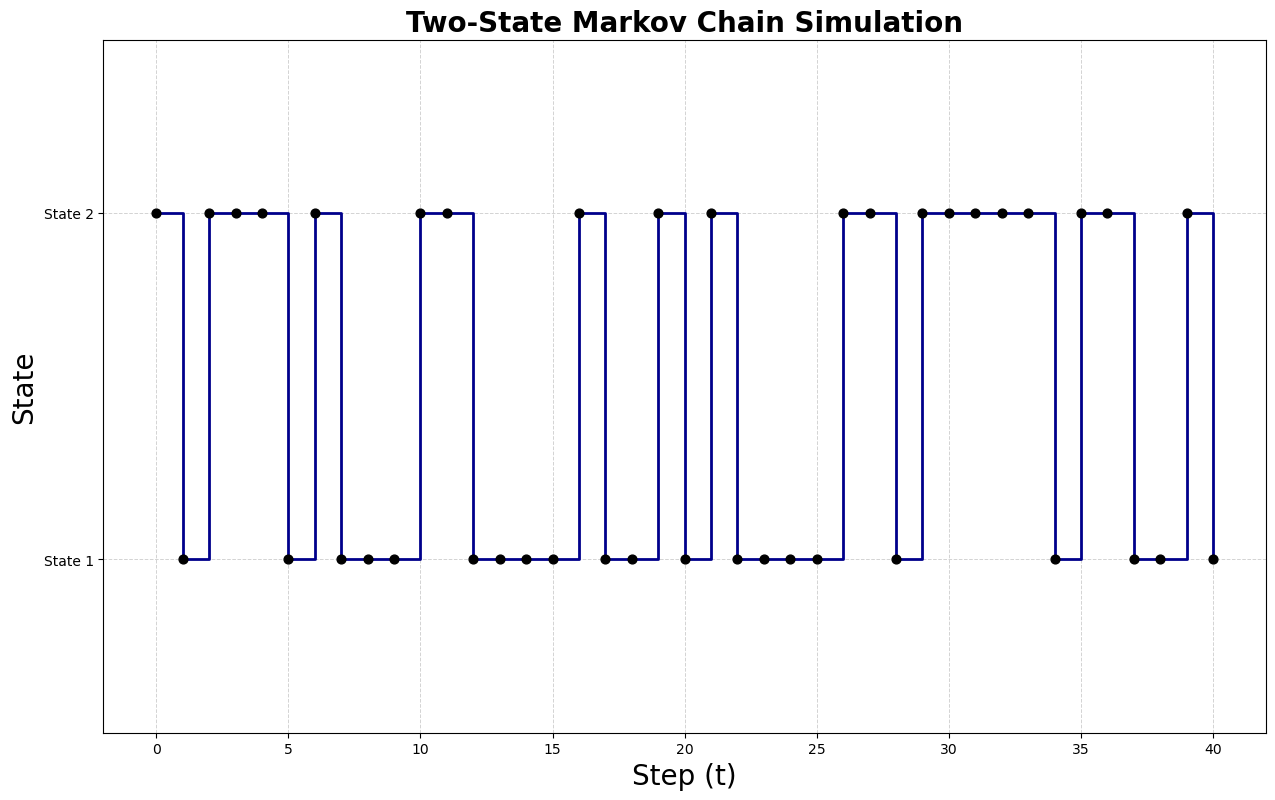
\includegraphics[width=0.9\textwidth]{chapter2-part2-plot1.png}

\vspace{3mm}
\textbf{Simulated trajectory of a 2-state Markov Chain with $n=40$.}
\end{frame}

% --------------------------
% Slide 23: Simulating a Markov Chain
% --------------------------
\begin{frame}{Markov Chain - Remarks}
\textbf{Remarks}:
\begin{itemize}
    \item The code shown before is not the most compact/efficient for the generation of Markov Chain paths.
    \item A more efficient approach is to use \textbf{categorical sampling}: 
    \begin{itemize}
        \item In \textbf{R}: use \texttt{sample()} or \texttt{rmultinom()}.
        \item In \textbf{Python}: use \texttt{numpy.random.choice()} (or 			 \texttt{torch.multinomial()} for GPU).
    \end{itemize}
    \item \textbf{Complexity:} generating a single path of length $n$ requires $O(n)$ categorical draws. The vectorized implementations are much faster when simulating many independent paths.
    \item Efficient Markov Chain simulation is especially important in \textbf{MCMC} (Markov Chain Monte Carlo), 
    where one often needs to generate millions of steps or multiple chains.
\end{itemize}
\end{frame}

% --------------------------
% Slide 24: Homework
% --------------------------
\begin{frame}{Homework}
Consider a Markov Chain taking values in $S=\left\{ 1,2, 3\right\}$ with initial distribution $X_0=2$ and
\begin{equation*}
P=\left[ \begin{array}{ccc} 0.2 & 0.5 & 0.3\\ 0.1 & 0.3 & 0.6\\
0.5 & 0.1 & 0.4 \end{array}\right]
\end{equation*}
Generate a path of this Markov Chain with length $n=40$.
\end{frame}

\end{document}